% !TEX root = ../main.tex
\section*{2}
\subsection*{a}

Because $p \in A$ and $q \in B$ where ${A,B}$ is a pair in the $s$-WSPD, the distance $|pq|$ should be large. In particular, $|pq| \geq sr$ where $r$ is the radius of $A$ and $B$. As we know, $s > 2$, so $sr > d$ where $d = 2s$ is the diameter of the circles. \\

If there is another point $p'$ in $A$, then $|pp'| \leq d < sr < |pq|$. Thus $q$ is not the nearest neighbor of $p$ anymore. This contradicts our proposal, which completes the proof.\\

If $p$ and $q$ are the closest pair in $P$, then $q$ is the nearest neighbor of $p$ and vice versa. Thus if $p \in A$ and $q \in B$ where ${A,B}$ is a pair in the $s$-WSPD, $A$ and $B$ contain only 1 element as being proven above. From the lecture, we know that the number of pairs in the $s$-WSPD is $O(s^d n)$. $s$ and $d$ do not depend on $n$, so we can consider this as $O(n)$. Therefore, in $O(n)$ time, we can extract all pairs ${A_i, B_i}$ in which both groups contain only 1 element. Then we can compare the distances between the items in each pair, and pick the one with the smallest distance, which also takes $O(n)$ because the number of such pairs is at most the number of the $s$-WSPD. In general, we can do that in $O(n)$ time.\\

\subsection*{b}
According to (a) if $s > 2$, for each point $p$ there will be a pair ${A,B} \in WSPD$ in which $A$ contains only $p$.
Thus, we have $n$ such circles $A$. Therefore, the number of pairs between the circles is at least $n/2$. \\

In the construction of a $t$-spanner, we use $s = 4(t + 1) / (t - 1)$. From this, we see that when $t > 1$, $s > 4$.
In the spanner, every vertex should be accessible, which means the number of edges
should be at least $n - 1$, otherwise there is at least an unreachable vertex.
The construction algorithm builds an edge in the spanner if there is a pair in
the $s$-WSPD. Therefore, the number of pairs should be at least $n - 1$, when $s > 4$. \\

\subsection*{c}
As we observe from (a), each point in P will have its own circle.
If $s > 0$, it means all circles with the same size are disjoint. With this property,
the number of circles of a WSPD, $\sum{|A_i|+|B_i|}$, is maximum when the algorithm
can always find a pair of circles with exactly 2 smaller circles inside.
Note that, if there are more than 2 smaller circles in a circle, the total number of circles reduces. \\

\begin{center}
    \label{figure1}
    \begin{figure}[h]
    \centering
    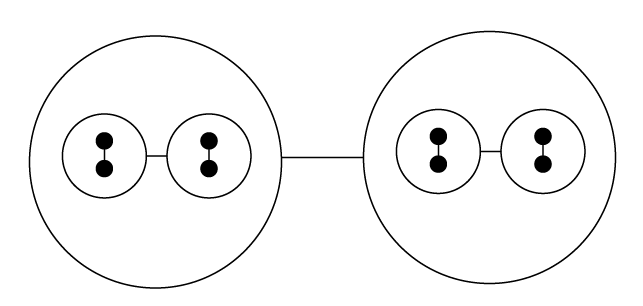
\includegraphics[width=5cm]{wspd}\\
    \caption{A WSPD whose circles contains 2 smaller circles.} \label{fig:wspd}
    \end{figure}
\end{center}

It is obvious to see that if every circle of the WSPD contains exactly 2 smaller circles,
the relation of circles is similar to binary tree whose leaves are the points of P. Hence, \\

\begin{align*}
    \text{No. Circles in the WSPD} &\leq \text{No. Nodes in the tree} - 1 \\
    &= O(n\log{n})
\end{align*}

Therefore, this proves $\sum{|A_i|+|B_i|} = O(n\log{n})$.
